%----------------------------------------------------------------------
% Problem 4

\begingroup
\allowdisplaybreaks

\newpage
\section{Problem 4}

\begin{figure}[h]
	\centering
	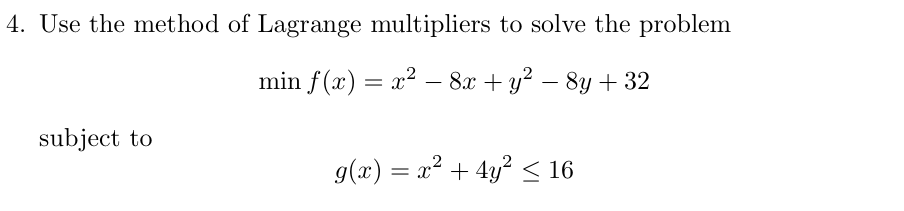
\includegraphics[width=0.8\textwidth]{./images/prob4_statement_1.png}
\end{figure}
\begin{figure}[h]
	\centering
	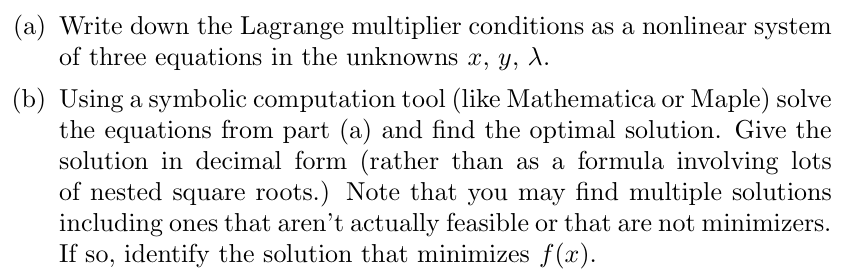
\includegraphics[width=0.8\textwidth]{./images/prob4_statement_2.png}
\end{figure}

\subsection{Solution}

\subsubsection{Part A}

Let the vector $\bv{x}$ consist of two elements $x,\,y$. The gradient of the objective function $f(\bv{x}) = x^2 - 8x + y^2 - 8y + 32$ is

\begin{align*}
	\nabla f (\bv{x}) = \begin{bmatrix} \frac{\partial f (\bv{x})}{\partial x} \\ \\ \frac{\partial f (\bv{x})}{\partial y} \end{bmatrix} = \begin{bmatrix} 2 x - 8 \\ \\ 2 y - 8 \end{bmatrix}
\end{align*}

The constraint $g(\bv{x}) = x^2 + 4y^2 \leq 16$ implies that the local minimization must satisfy the following system of equations. 

\begin{align*}
	\nabla f(\bv{x}) + \lambda \nabla g(\bv{x}) &= \bv{0} \\
	\\
	\lambda g(\bv{x}) &= \bv{0} \\
	\\
	g(\bv{x}) &\leq \bv{0} \\
	\\
	\lambda &\geq 0
\end{align*}

Therefore, the constraint function $g(\bv{x})$ and its gradient are

\begin{align*}
	g(\bv{x}) &= x^2 + 4y^2 - 16 \\
	\\
	\nabla g (\bv{x}) &= \begin{bmatrix} \frac{\partial g (\bv{x})}{\partial x} \\ \\ \frac{\partial g (\bv{x})}{\partial y} \end{bmatrix} = \begin{bmatrix} 2x \\ \\ 8y \end{bmatrix}
\end{align*}

The resulting nonlinear system of equations for the Lagrange multiplier conditions for the three unknowns $x, \, y, \, \lambda$ as

\begin{align*}
	\begin{bmatrix} 2 x - 8 \\ \\ 2 y - 8 \end{bmatrix} + \lambda \begin{bmatrix} 2x \\ \\ 8y \end{bmatrix} &= \bv{0} \\
	\\
	\lambda x^2 + \lambda 4 y^2 - 16 \lambda &= 0 
\end{align*}

for $g(\bv{x}) \leq \bv{0}, \, \lambda \geq 0$. Restating this system as scalar equations results in the final form used for evaluation via a symbolic solver. 

\begin{align*}
	2x + 2 \lambda x - 8 &= 0 \\
	\\
	2y + 2 \lambda y - 8 &= 0 \\
	\\
	\lambda x^2 + \lambda 4 y^2 - 16 \lambda &= 0 
\end{align*}


\subsubsection{Part B}

The symbolic toolbox in \MATLAB was utilized to solve the system of nonlinear equations. The code itself was executed in a live script for easy reading, and will be included in the homework submission for reference. 

Figure \ref{fig: matlab solver screenshot} contains a screenshot of the \MATLAB code used to solve the system of nonlinear equations. 

\begin{figure}[h] \label{fig: matlab solver screenshot}
	\centering
	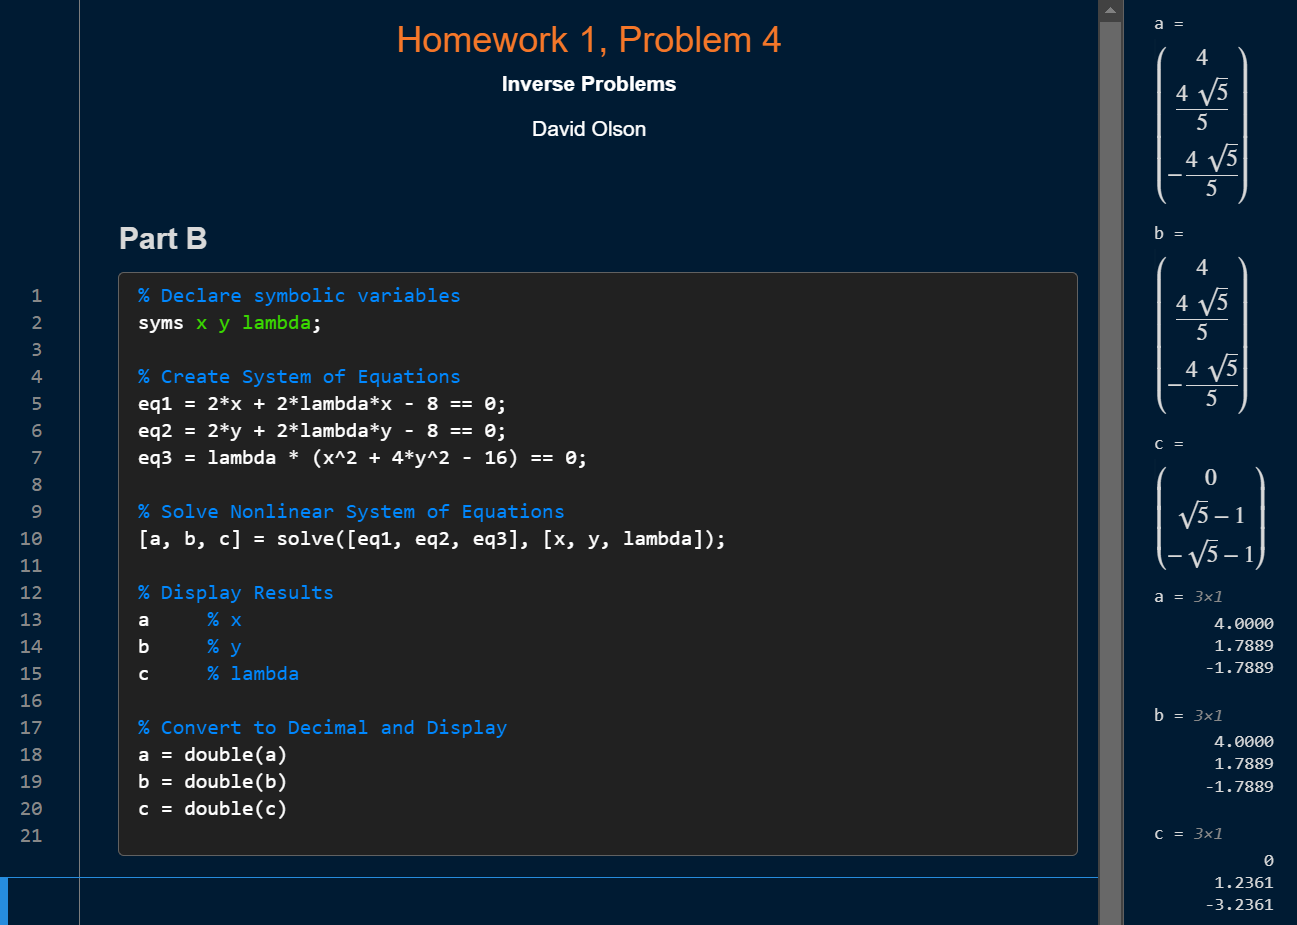
\includegraphics[width=0.95\textwidth]{./images/prob4_solver_screenshot.png}
	\caption{\MATLAB Solver Screenshot}
\end{figure}
\FloatBarrier

Each row of the three variables $\texttt{a}$, $\texttt{b}$, and $\texttt{c}$ correspond to one of three solutions to the system of equations. For convenience, each of these solutions were evaluated in \MATLAB to ensure the conditions $g(\bv{x}) \leq \bv{0}, \, \lambda \geq 0$ are met.

\begin{figure}[h] \label{fig: matlab eval screenshot}
	\centering
	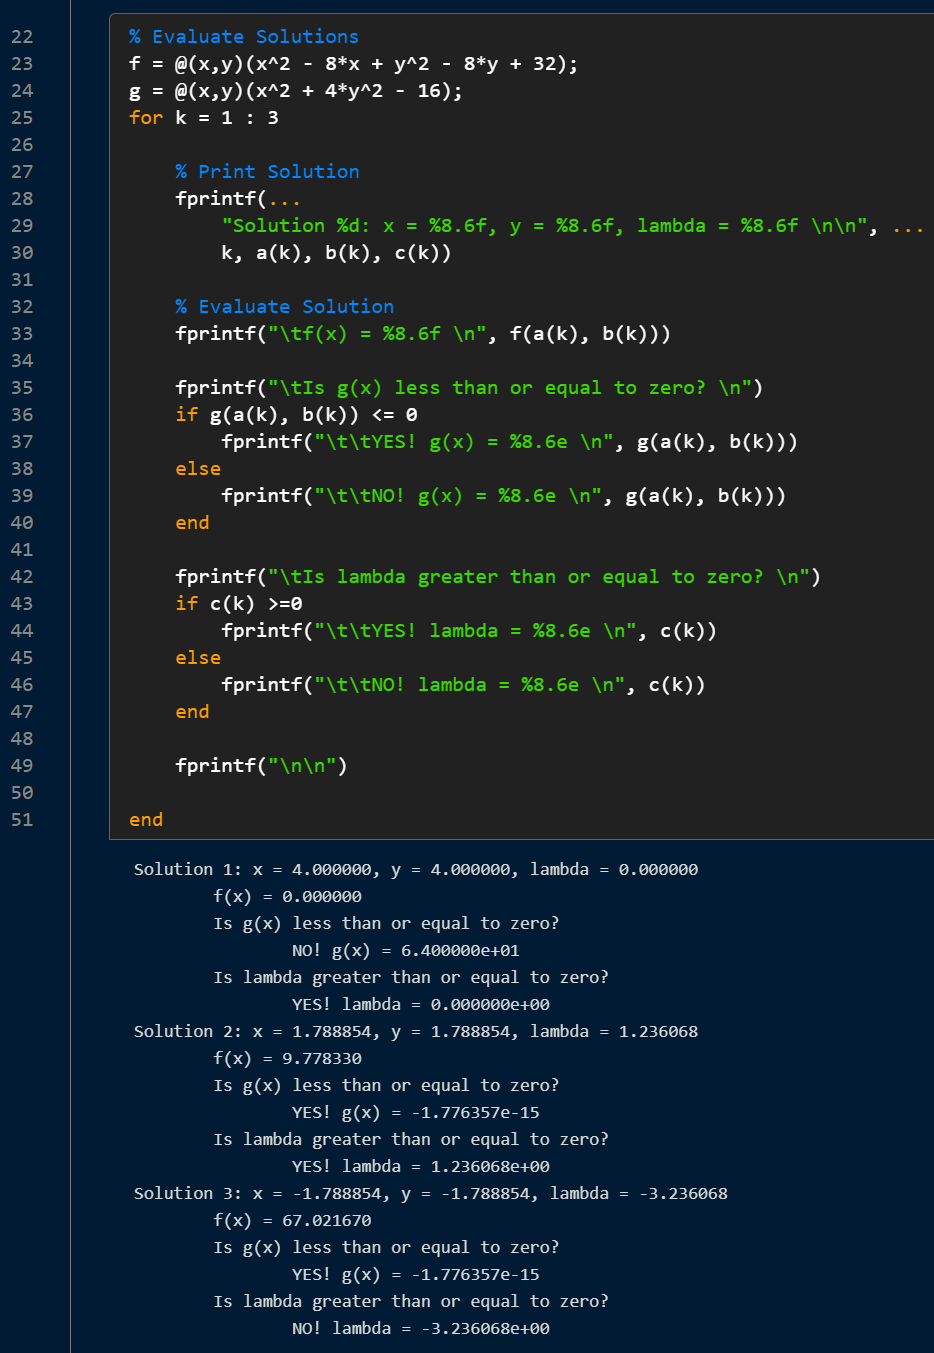
\includegraphics[width=0.8\textwidth]{./images/prob4_eval_screenshot.png}
	\caption{\MATLAB Evaluation Screenshot}
\end{figure}
\FloatBarrier

In summary, the only one of three solutions to the system of nonlinear equation that meets all conditions is

\begin{align*}
	x = \textrm{1.788854}, \,\,\, y = \textrm{1.788854}, \,\,\, \lambda = \textrm{1.236068}
\end{align*}

